\documentclass[11pt]{article}
\usepackage [french]{babel}
\usepackage [T1]{fontenc}

\usepackage[linesnumbered, ruled, french, onelanguage]{algorithm2e}
\usepackage{amssymb}
\usepackage{amsmath}
\usepackage{adjustbox}
\usepackage{graphicx}




\author{}
\title{Ray-Tracer}
\date{}

\begin{document}
\maketitle

\section{Détail des parties techniques}
\subsection{Le Ray Tracer}
Dans notre vie quotidienne, nous voyons ce qui nous entoure grâce aux photons émis par les différentes sources de lumière présentent autour de nous (le soleil ou nos lumières artificielles notamment). Chaque photon émit par ces sources vient alors frapper un des objets qui fait notre environnement. Si l'on imagine par exemple une tasse en face de nous, avec une lampe au plafond, un photon partant de cette dernière viendra rebondir sur la tasse pour ensuite, éventuellement, être redirigé en direction de nos yeux. Si le photon arrive en effet jusqu'à nos yeux, c'est alors qu'on verra se dessiner la tasse devant nous. La tasse est éclairée et nous la voyons. Bien sûr, ce phénomène est, à l'échelle de l'humain, instantané et c'est pour cela que nous ne voyons pas notre environnement apparaître progressivement devant nous chaque fois que nous allumons notre lumière. \\
L'objectif d'un algorithme de ray-tracing est de calculer le rendu d'une scène 3D d'une façon similaire à celle qui nous permet de voir tous les jours. En effet, nous pouvons faire un parallèle entre notre algorithme de ray-tracing et la vie à laquelle nous sommes habitués grâce à 3 composants principaux:
\begin{itemize}
	\item{Une scène composée d'objets (sphères, plans, triangles, ...) que l'on peut comparer à notre environnement}
	\item{Une (ou plusieures sources de lumière) jouant le même rôle que nos sources de lumière habituelles}
	\item{Une caméra représentant nos yeux}
\end{itemize}
Une différence notable avec ce qui nous permet de voir dans la vie de tous les jours est que nos rayons (ou photons) partiront de la caméra (nos yeux) plutôt que de la source de lumière. Nous faisons en quelque sorte le chemin inverse. En lançant un rayon au travers de chaque pixel de l'image que nous voulons calculer, nous pourrons ensuite vérifier si le rayon a rencontré un objet de la scène. Dans ce cas, le pixel pourra alors être coloré de la couleur de l'objet, le rendant ainsi visible.

\begin {algorithm}[H]
	\DontPrintSemicolon
	\KwIn{\textit{height} la hauteur de l'image à rendre\\\textit{width} la largeur de l'image\\\textit{scene} la scène 3D à rendre}
	\KwOut{P un ensemble de pixels $p_{i, j}$ $\{p_{0, 0}, p_{0, 1}, \ldots, p_{height-1, width-1}\}$, $i$, $j \in \mathbb{N}$, $0 \leqslant i \leqslant height-1$, $0 \leqslant j \leqslant width-1$\\\hfill\\}

	$O \gets Origine\ de\ la\ caméra$\\
	\For {$y \gets 0$ \textbf{to} $height$} 
	{
		\For {$x \gets 0$ \textbf{to} $width$} 
		{
			$C_{y, x} \gets convPxCoToWorldCoords(x, y)$\\
			$\overrightarrow{ray} \gets \overrightarrow{OC_{y,x}}$\\
			\hfill\\
			$p_{y, x} \gets lancerRayon(\overrightarrow{ray}, scene)$
		}
	}

	\caption{Pseudo-code du lancer des rayons}
	\label{lancerRayons}
\end {algorithm}

Comme le montre l'algorithme \ref{lancerRayons}, parcourir chaque pixel ne suffit pas. Si l'on souhaite lancer un rayon depuis la caméra à travers le pixel que l'on chercher à colorer, il nous faut les coordoonnées de ce pixel exprimées dans l'espace de la scène 3D.\\
Prenons l'exemple du rendu d'une image dans une résolution 800x600 pixels. Si l'on veut calculer la couleur du pixel de coordonnées $P = (430, 256)$ sur l'image, construire un rayon d'origine $O$ la caméra et de direction le vecteur $\overrightarrow{d} = \overrightarrow{OP}$, n'est pas une solution viable. En effet, le point $P$ n'est pas exprimé dans les coordonnées de notre scène où se trouvent nos objets. Il est exprimé dans les coordonnées de l'image. Nous avons donc besoin de faire correspondre les coordoonnées d'un pixel de l'image à ses coordoonnées dans le monde:

\begin {algorithm}[H]
	\DontPrintSemicolon
	\KwIn{$x, y \in \mathbb{N}, Pixel = (x, y)$ ;\\
		$width, height$\ la\ largeur\ et\ la\ hauteur\ de\ l'image\ à\ rendre\\
		$F \in ]0; 180[$\ le\ champ\ de\ vision\ de\ la\ caméra\ (FOV)}
	\KwOut{$P_{world}(x_{world}, y_{world}, -1)$\\les\ coordonnées\ du\ pixel\ exprimées\ dans\ l'espace\ de\ la\ scène\\\hfill\\}

	$aspectRatio \gets width/height$\\
	$demiPlaneHeight \gets tan(\frac{F}{2})$\\
	\hfill\\
	$x_{world} \gets x$\\
	$y_{world} \gets y$\\
	\hfill\\
	$x_{world} \gets (x_{world} +0.5) / width$\\
	$x_{world} \gets x_{world} * 2 -1$\\
	$x_{world} \gets x_{world} * aspectRatio$\\
	$x_{world} \gets x_{world} * demiPlaneHeight$\\

	\hfill\\
	$y_{world} \gets (y_{world} +0.5) / height$\\
	$y_{world} \gets 1 - y_{world} * 2$\\
	$y_{world} \gets y_{world} * demiPlaneHeight$\\

	\hfill\\
	\Return{$(x_{world}, y_{world}, -1)$}

	\caption{Conversion des coordonnées d'un pixel de l'image aux coordonnées de la scène}
	\label{conversionPixel}
\end{algorithm}

Il est important de remarquer que notre caméra se trouve initialement aux coordonnées $O = (0, 0, 0)$ et que sa direction de regard est $\overrightarrow{d_{cam}} = (0, 0, -1)$. Par convention, la grille de pixel virtuelle à travers laquelle nous faisons passer nos rayons se trouve à 1 unité de distance de la caméra, dans sa direction de regard. Ainsi, la coordonnée z des pixels sera toujours -1.\\
\adjustbox{center}{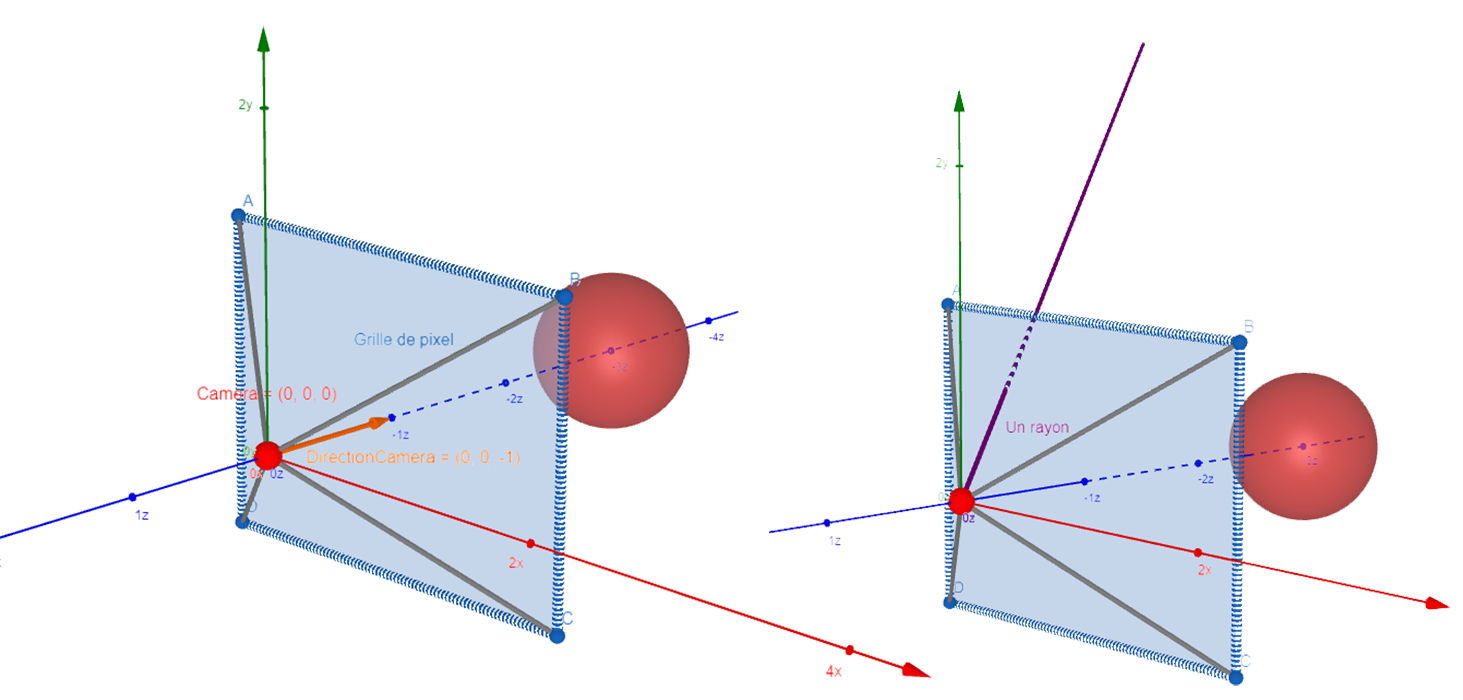
\includegraphics[width=1.4\textwidth]{img/rt/final/repre_cam_rayon.png}}
En reprenant l'exemple de notre image de rendu en 800x600 pixels:\\
$P(x, y, z), x \in [0, 799], y \in [0, 599], z = -1$ :
\begin{enumerate}
	\item{}
\end{enumerate}
Il faut cependant convertir les coordonnées des pixels en les coordonnées du monde, présenter un algo de la méthode et refaire l'algo 1 pour dire comment il a évolué (juste rajouter la ligne qui permet de convertir les co des pixels). 
Maintenant qu'on a la conversion des pixels et le ray tracing basique de chaque pixel, présenter la méthode lancerRayon la plus simple, juste pour expliquer comment on obtient les couleurs et montrer que l'image obtenue est pas ouffissime, toute plate

--> enchaîner sur l'ombrage de Phong:
	- Dire que l'image est pas ouf, en effet, pas de lumière tout ça tout ça
	- Dire en quoi consiste l'ombrage de phong
	- PRésenter comment on calcule chaque composante
	- Une image séparée pour chaque composante + l'image résultatn de toutes les composantes en même temps

A la fin de ce processus, nous obtenons notre première image 

\section{Structuration du projet}
\subsection{Les packages}
\subsubsection{Liés au Ray Tracer}




\end{document}